\section{Thực nghiệm và kết quả}

Toàn bộ các mô hình sau khi huấn luyện và tinh chỉnh siêu tham số được đánh giá độc lập trên cùng một tập kiểm thử (\textit{Test Set}) gồm 4.698 mẫu đã được phân tầng.

\subsection{So sánh tổng hợp các mô hình}
Bảng~\ref{tab:final_comparison} tổng hợp hiệu năng của tất cả các mô hình học máy được triển khai trong nghiên cứu, sắp xếp giảm dần theo chỉ số mục tiêu Macro-F1.

\begin{table}[H]
\centering
\small
\setlength{\tabcolsep}{3.8pt}
\begin{tabular}{|l|c|c|c|c|c|c|c|}
\hline
\textbf{Mô hình} & \textbf{Accuracy} & \textbf{F1 (Lớp 1)} & \textbf{F1 (Lớp 0)} & \textbf{Macro-F1} & \textbf{Recall (Lớp 0)} & \textbf{ROC-AUC} & \textbf{Fit Time (s)} \\ \hline
\textbf{LogReg (tuned)} & \textbf{0.9106} & \textbf{0.9450} & 0.7605 & \textbf{0.8528} & 0.7988 & 0.9478 & 2.86 \\ \hline
LogReg (baseline) & 0.9044 & 0.9402 & \textbf{0.7618} & 0.8510 & \textbf{0.8599} & \textbf{0.9501} & 3.32 \\ \hline
XGBoost (tuned) & 0.9059 & 0.9418 & 0.7553 & 0.8485 & 0.8168 & 0.9444 & 8.91 \\ \hline
XGBoost + metadata & 0.9051 & 0.9413 & 0.7517 & 0.8465 & 0.8084 & 0.9443 & 10.40 \\ \hline
XGBoost (baseline) & 0.8995 & 0.9376 & 0.7415 & 0.8396 & 0.8108 & 0.9419 & 6.87 \\ \hline
NaiveBayes (tuned) & 0.9017 & 0.9407 & 0.7116 & 0.8262 & 0.6826 & 0.9445 & 3.76 \\ \hline
NaiveBayes (baseline) & 0.9040 & 0.9433 & 0.6879 & 0.8156 & 0.5952 & 0.9484 & \textbf{1.21} \\ \hline
SVM (Bagging + Sigmoid) & 0.9000 & 0.9400 & 0.6600 & 0.8000 & 0.5700 & -- & 17.57 \\ \hline
\end{tabular}
\caption{Bảng so sánh tổng hợp hiệu năng các mô hình trên tập kiểm thử}
\label{tab:final_comparison}
\end{table}

\begin{figure}[H]
\centering
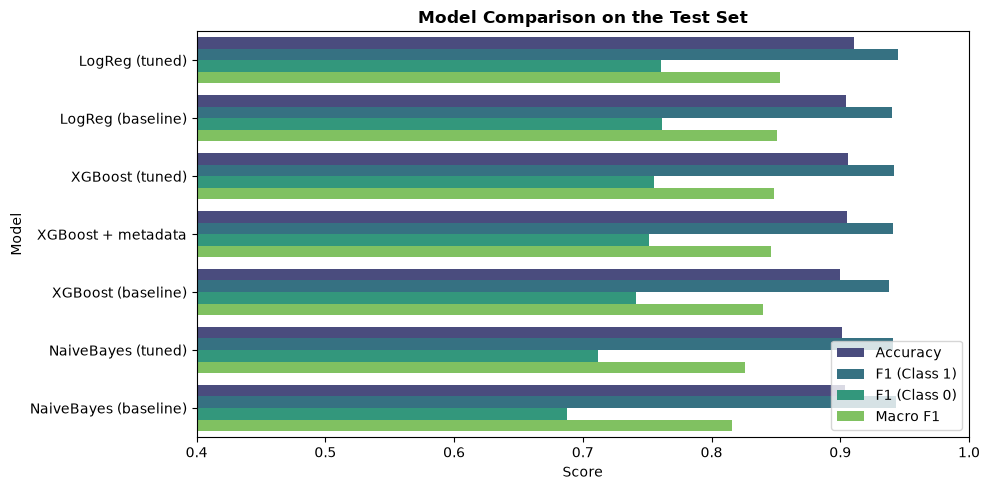
\includegraphics[width=0.85\textwidth]{figures/logreg_xgb_cell33_1.png}
\caption{Biểu đồ so sánh các chỉ số hiệu năng giữa các mô hình trên tập kiểm thử}
\label{fig:model_comparison}
\end{figure}

Từ Bảng~\ref{tab:final_comparison} và Hình~\ref{fig:model_comparison}, Logistic Regression sau khi tinh chỉnh đạt Macro-F1 cao nhất (0.8528) và thời gian huấn luyện nhanh (2.86 giây). XGBoost sau tuning đạt hiệu năng rất cạnh tranh (Macro-F1 0.8485, Recall lớp 0 đạt 0.8168). Các mô hình Naive Bayes và SVM hoàn chỉnh đạt độ chính xác Accuracy xấp xỉ 90\% nhưng có F1 và Recall trên lớp thiểu số thấp hơn.

\subsection{Phân tích hiện tượng quá khớp (Overfitting Analysis)}
Khoảng cách sai lệch giữa điểm Macro-F1 trên tập huấn luyện (\textit{train}) và tập kiểm thử (\textit{test}) được sử dụng làm thước đo phát hiện nguy cơ quá khớp:
\begin{equation}
\text{Gap} = \text{Macro-F1}_{\text{train}} - \text{Macro-F1}_{\text{test}}
\end{equation}

\begin{table}[H]
\centering
\begin{tabular}{|l|c|c|c|}
\hline
\textbf{Mô hình} & \textbf{Macro-F1 (Train)} & \textbf{Macro-F1 (Test)} & \textbf{Gap (Train - Test)} \\ \hline
NaiveBayes (baseline) & 0.9557 & 0.8156 & 0.1401 \\ \hline
LogReg (tuned) & 0.9562 & 0.8528 & 0.1034 \\ \hline
XGBoost + metadata & 0.9330 & 0.8465 & 0.0866 \\ \hline
XGBoost (baseline) & 0.9251 & 0.8396 & 0.0855 \\ \hline
XGBoost (tuned) & 0.9327 & 0.8485 & 0.0842 \\ \hline
NaiveBayes (tuned) & 0.8904 & 0.8262 & 0.0642 \\ \hline
LogReg (baseline) & 0.9068 & 0.8510 & \textbf{0.0558} \\ \hline
\end{tabular}
\caption{So sánh Macro-F1 giữa tập huấn luyện và tập kiểm thử (Khoảng cách Gap)}
\label{tab:overfitting_gap}
\end{table}

Kết quả ở Bảng~\ref{tab:overfitting_gap} cho thấy Naive Bayes baseline có độ chênh lệch lớn nhất (0.1401) do chưa được tối ưu hóa tham số làm trơn $\alpha$. Ngược lại, sau khi tinh chỉnh siêu tham số, khoảng cách sai lệch của Naive Bayes giảm xuống còn 0.0642. Đối với XGBoost, việc kiểm soát độ sâu cây (\texttt{max\_depth=7}), tỷ lệ lấy mẫu con (\texttt{subsample=0.9315}, \texttt{colsample=0.4271}) và trọng số lá tối thiểu (\texttt{min\_child\_weight=2}) giữ khoảng cách ở mức an toàn ($0.0842 \div 0.0866$). Logistic Regression baseline đạt độ ổn định cao nhất với Gap chỉ 0.0558.

\subsection{Ma trận nhầm lẫn và Báo cáo phân loại}
Hình~\ref{fig:conf_matrices} thể hiện ma trận nhầm lẫn của 4 mô hình dẫn đầu trên tập kiểm thử (gồm 835 mẫu lớp 0 và 3.863 mẫu lớp 1).

\begin{figure}[H]
\centering
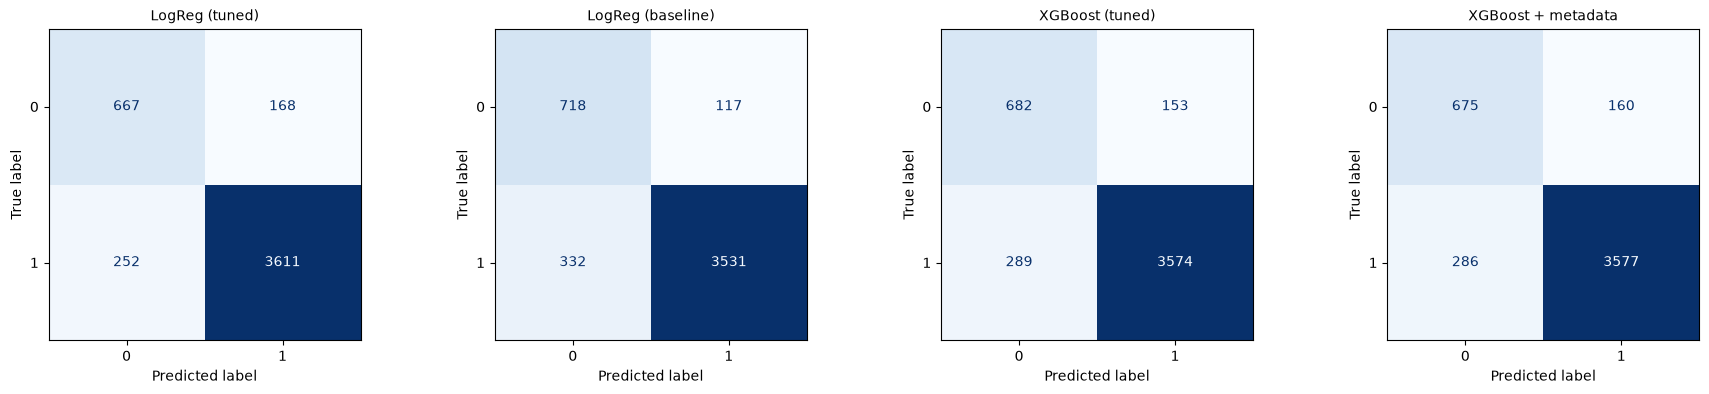
\includegraphics[width=0.95\textwidth]{figures/logreg_xgb_cell37_0.png}
\caption{Ma trận nhầm lẫn của 4 mô hình đạt hiệu năng Macro-F1 hàng đầu}
\label{fig:conf_matrices}
\end{figure}

Báo cáo phân loại chi tiết của mô hình tốt nhất (Logistic Regression sau tinh chỉnh) được trình bày trong Bảng~\ref{tab:best_report}.

\begin{table}[H]
\centering
\begin{tabular}{|l|c|c|c|c|}
\hline
\textbf{Lớp phân loại} & \textbf{Precision} & \textbf{Recall} & \textbf{F1-Score} & \textbf{Hỗ trợ (Support)} \\ \hline
Không đề xuất (Lớp 0) & 0.73 & 0.80 & 0.76 & 835 \\ \hline
Có đề xuất (Lớp 1)    & 0.96 & 0.93 & 0.95 & 3.863 \\ \hline
\textbf{Accuracy}     & \multicolumn{3}{c|}{0.91} & 4.698 \\ \hline
\textbf{Macro Avg}    & 0.84 & 0.87 & 0.85 & 4.698 \\ \hline
\textbf{Weighted Avg} & 0.91 & 0.91 & 0.91 & 4.698 \\ \hline
\end{tabular}
\caption{Báo cáo phân loại chi tiết của mô hình Logistic Regression (tuned)}
\label{tab:best_report}
\end{table}

\subsection{Các từ có ảnh hưởng lớn nhất (Most Influential Terms)}
Dựa trên hệ số hồi quy $w$ của mô hình Logistic Regression tối ưu:
\begin{itemize}
    \item \textbf{Hệ số âm}: Đẩy xác suất dự đoán về phía nhãn 0 (Không đề xuất).
    \item \textbf{Hệ số dương}: Đẩy xác suất dự đoán về phía nhãn 1 (Có đề xuất).
\end{itemize}

\begin{figure}[H]
\centering
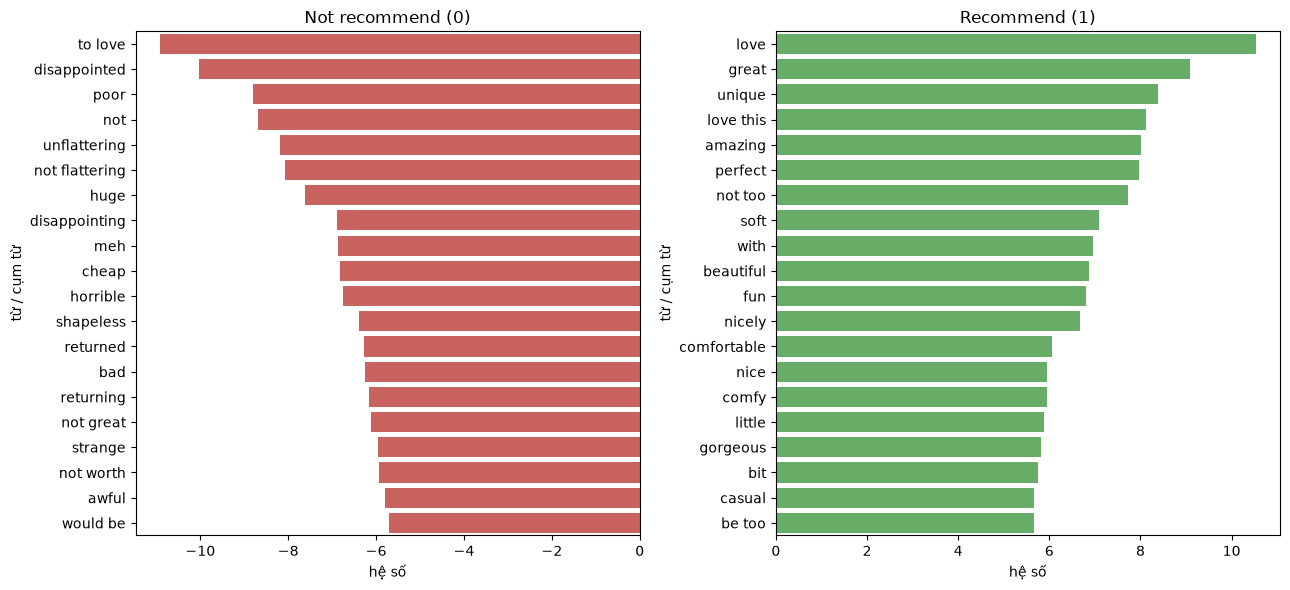
\includegraphics[width=0.92\textwidth]{figures/logreg_xgb_cell39_0.png}
\caption{Top 20 từ/cụm từ có hệ số ảnh hưởng mạnh nhất đến quyết định phân loại của Logistic Regression}
\label{fig:top_terms}
\end{figure}

Hình~\ref{fig:top_terms} cho thấy các từ chỉ sự thất vọng về phom dáng, chất lượng hoặc hành vi trả hàng mang trọng số âm lớn nhất: \textit{huge}, \textit{unflattering}, \textit{returned}, \textit{returning}, \textit{cheap}, \textit{disappointed}, \textit{poorly}, \textit{boxy}. Ngược lại, các từ thể hiện sự hài lòng cao mang trọng số dương lớn nhất: \textit{love}, \textit{great}, \textit{perfect}, \textit{compliments}, \textit{comfortable}, \textit{flattering}, \textit{soft}.

\subsection{Phân tích lỗi dự đoán (Error Analysis)}
Khảo sát các trường hợp mô hình phân loại sai với độ tự tin dự đoán cao nhất ($P(\text{recommend})$ gần 0 hoặc 1) chỉ ra hai nguyên nhân chính:
\begin{enumerate}
    \item \textbf{Thực tế KHÔNG đề xuất (0) nhưng mô hình dự đoán đề xuất (1) ($P \approx 0.99 \div 1.0$)}:
    \begin{itemize}
        \item Khách hàng mở đầu bằng khen ngợi tổng quát hoặc kiểu dáng nhưng gặp vấn đề về kích cỡ/đường may buộc phải trả lại: ví dụ đánh giá \textit{``Love this dress I also have this dress in 3/4...''} hoặc \textit{``Cute pant Unfortunately i had to size down twice...''}.
        \item Mô hình dựa trên túi từ (Bag-of-Words/TF-IDF) bắt gặp các từ tích cực mạnh (\textit{love}, \textit{cute}, \textit{beautiful}) nhưng không bắt được ngữ cảnh đảo ngược của từ nối (\textit{unfortunately}, \textit{however}).
    \end{itemize}
    \item \textbf{Thực tế CÓ đề xuất (1) nhưng mô hình dự đoán không đề xuất (0) ($P \le 0.008$)}:
    \begin{itemize}
        \item Khách hàng đánh giá tiêu đề mang tính cảnh báo hoặc chê chi tiết phụ nhưng tổng thể vẫn hài lòng và đồng ý giới thiệu: ví dụ \textit{``Much thinner I was so excited...''}, \textit{``Great dress, poor stitching...''}, \textit{``I recommend with caveats...''}.
        \item Sự xuất hiện của các từ mang trọng số âm mạnh (\textit{terrible}, \textit{poor}, \textit{thinner}) khiến mô hình hạ thấp xác suất dự đoán.
    \end{itemize}
\end{enumerate}

\section{Thảo luận}

Dựa trên kết quả thực nghiệm, nhóm rút ra các nhận xét chuyên sâu:
\begin{enumerate}
    \item \textbf{Ý nghĩa của các thước đo đánh giá}: Độ chính xác (Accuracy) có sự khác biệt rất nhỏ giữa các mô hình (đều dao động quanh 90\% $\div$ 91\%), trong khi Macro-F1 và Recall của lớp 0 phản ánh rõ nét khả năng nhận diện lớp thiểu số. Điều này chứng minh việc chọn Macro-F1 làm mục tiêu tối ưu là hoàn toàn đúng đắn.
    \item \textbf{Hiệu năng giữa mô hình tuyến tính và mô hình cây}: Logistic Regression sau khi tinh chỉnh siêu tham số đạt Macro-F1 cao nhất (0.8528) với thời gian huấn luyện chỉ 2.86 giây. Mặc dù XGBoost là mô hình phi tuyến mạnh mẽ và có hỗ trợ tăng tốc GPU, hiệu năng của XGBoost (0.8485) không vượt qua mô hình tuyến tính trên không gian đặc trưng TF-IDF thưa và nhiều chiều. Hiện tượng này phù hợp với lý thuyết học máy cho dữ liệu văn bản: các ranh giới quyết định tuyến tính trong không gian thưa nhiều chiều thường mang lại tính tổng quát hóa cao và ít bị ảnh hưởng bởi nhiễu cục bộ.
    \item \textbf{Độ chênh lệch giữa các mô hình dẫn đầu}: Chênh lệch Macro-F1 giữa Logistic Regression và XGBoost là tương đối nhỏ (khoảng 0.004). Sự sai khác này có thể chịu ảnh hưởng từ cách phân chia ngẫu nhiên một lần tập dữ liệu (\textit{single train-test split}). Cần tiến hành đánh giá lặp lại nhiều lần để có kết luận khái quát hơn.
    \item \textbf{Vai trò của siêu dữ liệu (Metadata)}: Việc bổ sung thông tin độ tuổi (\texttt{Age}) và danh mục sản phẩm (\texttt{Division}, \texttt{Department}, \texttt{Class}) không làm tăng hiệu năng của XGBoost (Macro-F1 đạt 0.8465 so với 0.8485 của XGBoost chỉ dùng văn bản). Điều này chứng minh tín hiệu quyết định khách hàng có đề xuất sản phẩm hay không tập trung chủ yếu trong nội dung cảm xúc của bài đánh giá, trong khi các thuộc tính nhân khẩu học và danh mục đóng góp rất ít thông tin phân biệt.
\end{enumerate}

\section{Kết luận và hướng phát triển}

\subsection{Kết luận}
Báo cáo đã hoàn thành trọn vẹn quy trình giải quyết bài toán phân loại đánh giá thời trang nữ theo đúng yêu cầu môn học Machine Learning:
\begin{itemize}
    \item Phân tích đặc điểm dữ liệu, nhận diện và xử lý triệt để hai thách thức cốt lõi: mất cân bằng lớp và rò rỉ mục tiêu từ thuộc tính \texttt{Rating}.
    \item Hiện thực và đánh giá 4 thuật toán học máy đại diện cho các trường phái khác nhau: Support Vector Machine, Logistic Regression, Multinomial Naive Bayes và XGBoost.
    \item Áp dụng thành công các kỹ thuật học máy nâng cao: lựa chọn đặc trưng (\textit{Feature Selection} qua Chi-Square/ANOVA), tối ưu siêu tham số (\textit{RandomizedSearchCV} với \textit{Stratified 5-Fold CV}), học kết hợp (\textit{Bagging/AdaBoost}) và tích hợp siêu dữ liệu đa phương thức (\textit{ColumnTransformer}).
    \item Mô hình Logistic Regression tối ưu đạt hiệu năng dẫn đầu với Macro-F1 đạt 0.8528, độ chính xác 91.06\% và thời gian thực thi ngắn.
\end{itemize}

\subsection{Hạn chế của đề tài}
\begin{itemize}
    \item Thí nghiệm chỉ thực hiện trên một lần phân chia train/test cố định; chưa tính toán khoảng tin cậy (\textit{confidence interval}) qua kiểm định lặp lại nhiều lần.
    \item Không gian siêu tham số và số vòng tìm kiếm ngẫu nhiên (\textit{n\_iter}) còn bị giới hạn bởi tài nguyên tính toán.
    \item Biểu diễn TF-IDF dạng túi từ chưa nắm bắt được ngữ cảnh trật tự từ khoảng cách xa, cấu trúc ngữ pháp phức tạp, ngữ cảnh phủ định đa tầng hoặc cách diễn đạt mỉa mai (\textit{sarcasm}).
    \item Ngưỡng quyết định xác suất đang được cố định ở mức mặc định 0.5, chưa được tối ưu hóa theo đường cong ROC hoặc bài toán chi phí thiệt hại cụ thể.
\end{itemize}

\subsection{Hướng phát triển}
\begin{itemize}
    \item Nghiên cứu và thử nghiệm các mô hình mạng nơ-ron hồi tiếp (BiLSTM, GRU) và mạng tích chập một chiều (1D-CNN) để biểu diễn chuỗi từ theo thứ tự thời gian.
    \item Ứng dụng các mô hình ngôn ngữ dựa trên kiến trúc Transformer tiền huấn luyện (BERT, RoBERTa, DistilBERT) nhằm nắm bắt sâu sắc ngữ cảnh hai chiều và ngữ nghĩa tiềm ẩn trong các bài đánh giá phức tạp.
    \item Tối ưu hóa ngưỡng cắt xác suất (\textit{Threshold Tuning}) kết hợp kỹ thuật tái lấy mẫu nâng cao (SMOTE, Focal Loss) nhằm gia tăng hơn nữa Recall của lớp khách hàng không đề xuất.
\end{itemize}

\begin{thebibliography}{99}
\bibitem{pedregosa2011}
Pedregosa, F., Varoquaux, G., Gramfort, A., Michel, V., Thirion, B., Grisel, O., Blondel, M., Prettenhofer, P., Weiss, R., Dubourg, V., Vanderplas, J., Passos, A., Cournapeau, D., Brucher, M., Perrot, M., Duchesnay, E. (2011). \textit{Scikit-learn: Machine Learning in Python}. Journal of Machine Learning Research, 12, 2825--2830.

\bibitem{chen2016}
Chen, T., Guestrin, C. (2016). \textit{XGBoost: A Scalable Tree Boosting System}. In Proceedings of the 22nd ACM SIGKDD International Conference on Knowledge Discovery and Data Mining (KDD '16), 785--794.

\bibitem{bergstra2012}
Bergstra, J., Bengio, Y. (2012). \textit{Random Search for Hyper-Parameter Optimization}. Journal of Machine Learning Research, 13, 281--305.

\bibitem{kaggle2018}
Agarap, A. F. (2018). \textit{Statistical Analysis on E-Commerce Reviews, with Sentiment Classification using Bidirectional Recurrent Neural Network (RNN)}. arXiv preprint arXiv:1805.03687.

\bibitem{dataset}
Women's E-Commerce Clothing Reviews Dataset. Kaggle. \url{https://www.kaggle.com/datasets/nicapotato/womens-ecommerce-clothing-reviews}.
\end{thebibliography}
